\documentclass[a4paper,12pt]{scrartcl}

%% Pacotes elementares
\usepackage[brazil]{babel}
\usepackage[utf8]{inputenc}
\usepackage[T1]{fontenc}
\usepackage{color}
\usepackage{amsmath,amssymb,amsmath,bbm,amsfonts}
\usepackage{graphicx}
\usepackage{url}
\usepackage{booktabs} % Formatação de tabelas

%%%%%%%%%%%%%%%%%%%%%%%%%%%%%%%%%%%%%%%%%%%%%%
% Configuração da página, espaçamento e fontes

\renewcommand{\titlefont}{\rmfamily\bfseries}
\renewcommand{\sectfont}{\normalsize\rmfamily\bfseries}
\renewcommand{\descfont}{\normalsize\rmfamily\bfseries}
\usepackage{anysize}
\marginsize{30mm}{20mm}{30mm}{20mm}
\usepackage[onehalfspacing]{setspace}
\addto\captionsbrazil{\renewcommand{\refname}{Referências Bibliográficas}}

%%%%%%%%%%%%%%%%%%%%%%%%%%%%%%%%%%%%%%%%%%%%%%
% Cabeçalhos e estilo

\usepackage[headsepline]{scrlayer-scrpage}
\setlength{\headheight}{1.1\baselineskip}
\automark[section]{section}
\clearpairofpagestyles
\ihead{\footnotesize{Núcleo de Computação\\
Escola Superior de Tecnologia\\
Universidade do Estado do Amazonas}}
\ohead{

\includegraphics[width=0.10\textwidth]{./img/logo_uea}

\includegraphics[width=0.12\textwidth]{./img/nucomp}}


\ifoot{}
\ofoot[\pagemark]{\pagemark}

%%%%%%%%%%%%%%%%%%%%%%%%%%%%%%%%%%%%%%%%%%%%%%
% Revisão e anotações
\usepackage{xcolor}
\definecolor{lightblue}{RGB}{0,191,255}
\usepackage[textsize=tiny,backgroundcolor=lightblue,linecolor=lightblue]{todonotes}


\begin{document}

\title{Manual do Aluno}
\subtitle{Guia de Elaboração do Trabalho de Conclusão de Curso}
\author{Núcleo de Computação\\ \multicolumn{1}{p{.7\textwidth}}{\centering\small{Escola Superior de Tecnologia\\Universidade do Estado do Amazonas\\Av. Darcy Vargas, 1200\\Manaus, Amazonas, Brasil}}}


\maketitle

\section*{Apresentação}

\todo{Escrever um texto de boas vindas ao manual do TCC, apresentando uma visão geral do documento e desejando força nesta etapa do trabalho. Utilizar uma linguagem fácil e amigável nesta apresentação.}

Exemplos de trabalhos orientados anteriormente permeiam este manual do aluno, auxiliando no entendimento dos elementos e conceitos apresentados.

\begin{flushright}
Com carinho,\\
Elloá B. Guedes (ebgcosta@uea.edu.br)\\
Flávio José Mendes Coelho (fcoelho@uea.edu.br)\\
Ricardo Rios (rrios@uea.edu.br)
\end{flushright}


\section{Introdução}

\section{Sugestões de Leitura}
Para que você se prepare adequadamente para o seu TCC, além de ler este manual e conhecer as regras e práticas adotadas no NUCOMP, nós sugerimos algumas leituras essenciais.

\noindent\begin{minipage}{0.8\textwidth}
\textbf{Título}. Metodologia de Pesquisa Em Ciência da Computação\\
\textbf{Autor}. Raul Wazlawick\\
\textbf{Editora}. Campus Elsevier\\
\textbf{Ano}. 2014\\
\end{minipage}\begin{minipage}{0.2\textwidth}
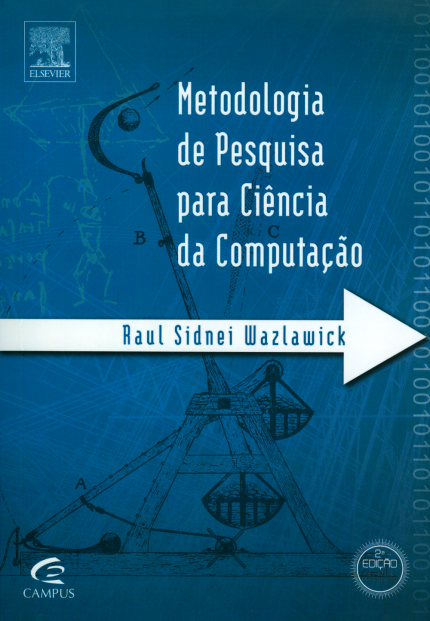
\includegraphics[width=\linewidth]{./img/wazlawick}
\end{minipage}

\noindent \begin{minipage}{0.8\textwidth}
\textbf{Título}. Guia Prático para Redação Científica\\
\textbf{Autor}. Gilson Volpato\\
\textbf{Editora}. Best Writing\\
\textbf{Ano}. 2015\\
\end{minipage}\begin{minipage}{0.2\textwidth}

\includegraphics[width=\linewidth]{./img/volpato}
\end{minipage}

\noindent \begin{minipage}{0.8\textwidth}
\textbf{Título}. Elaboração de Projeto, TCC, Dissertação e Tese \\
\textbf{Autor}. Mario de Souza Almeida\\
\textbf{Editora}. Atlas\\
\textbf{Ano}. 2014\\
\end{minipage}\begin{minipage}{0.2\textwidth}

\includegraphics[width=\linewidth]{./img/almeida}
\end{minipage}


\section{Objetivos do Trabalho de Conclusão de Curso}
Você é um guerreiro(a)! Venceu um vestibular concorrido, foi aprovado em uma faculdade pública, cursou muitas disciplinas, algumas delas extremamente desafiadoras, e está no passo final para a conclusão do seu curso, a realização do \emph{Trabalho de Conclusão de Curso} (TCC).

O TCC é um dos requisitos parciais para a sua graduação, juntamente com as disciplinas, atividades complementares, etc. É um \emph{trabalho individual} e de \emph{caráter monográfico}, ou seja, de natureza dissertativa que se destina a abordar um assunto em específico. O TCC tem basicamente três objetivos:

\begin{enumerate}
  \item Reunir, aprofundar e sistematizar os conteúdos disponibilizados ao longo das disciplinas do curso em um trabalho de caráter bibliográfico ou prático, relacionado à sua formação;
  \item Concentrar em uma atividade acadêmica as capacidades de criação e de pesquisa do acadêmico no que diz respeito à organização, metodologia, domínio das técnicas de pesquisa, processos de apresentação de trabalho, conhecimentos da pesquisa bibliográfica e da documentação, técnicas de coleta, análise e apresentação de dados, clareza e coerência na redação final;
  \item Contribuir para a criação e disseminação de conhecimento técnico e científico na Computação.
\end{enumerate}

Mas isto não será feito do dia para a noite. Para tanto, você contará com pelo menos três ferramentas essenciais: um orientador; e duas disciplinas (TCC1 e TCC2).

\subsection{Orientador}

\subsection{Disciplinas TCC1 e TCC2}


\section{Estrutura do Documento}
\subsection{Trabalho de Conclusão de Curso I}

\subsection{Trabalho de Conclusão de Curso II}


\section{Checklists}
\input{./files/checklists}




\bibliographystyle{abnt}
\bibliography{ref}

\end{document}
